\documentclass[14pt, a4paper, oneside]{extreport}

% ================= CÁC THƯ VIỆN CẦN THIẾT =================
\usepackage[utf8]{vietnam} % Hỗ trợ gõ tiếng Việt tốt nhất cho pdfLaTeX
\usepackage{amsmath, amssymb, amsfonts} % Hỗ trợ công thức và ký hiệu toán học
\usepackage[top=2cm, bottom=2cm, left=3cm, right=2cm]{geometry} % Căn lề chuẩn cho dự án
\usepackage{tikz} % Thư viện vẽ hình
\usepackage{pgfplots} % Thư viện vẽ đồ thị (Parabol, v.v.)
\pgfplotsset{compat=1.18} % Tương thích phiên bản pgfplots
\usepackage{graphicx} % Chèn hình ảnh (logo trường)
\usepackage{hyperref} % Tạo liên kết trong tài liệu
\usepackage{setspace} % Hỗ trợ giãn dòng
\setstretch{1.25} % Giãn dòng 1.25 cho dễ nhìn
\usepackage{amsmath, amssymb}
\usepackage[skins,breakable]{tcolorbox}
\usepackage{array}
\usepackage{enumitem}
\usepackage{tikz}

\begin{document}

% ================= TRANG BÌA =================
\begin{titlepage}
    \begin{center}
        \vspace*{1cm}
        
  
        \textbf{\large ỨNG DỤNG CNTT TRONG DẠY HỌC TOÁN} \\
        \vspace{0.5cm}
        \rule{0.6\textwidth}{0.5pt} % Đường kẻ ngang
        
        \vspace{2.5cm}
        
        % Nếu bạn có logo trường, hãy tải lên Overleaf và bỏ dấu % ở dòng dưới để chèn logo
        % \includegraphics[width=4cm]{ten_file_logo.png} 
        
        \vspace{2cm}
        
        \textbf{\LARGE DỰ ÁN LATEX CÁ NHÂN} \\
        \vspace{0.5cm}
        \textbf{\huge ỨNG DỤNG CỦA BẤT ĐẲNG THỨC BẬC HAI MỘT ẨN TRONG BÀI TOÁN THỰC TIỄN} \\
        
        \vspace{3cm}
        
       
            \begin{tabular}{ll}
               
                \textbf{Sinh viên thực hiện: Nguyễn Thị Xuân Thi} \\
                \textbf{Mã sinh viên: 23S101002} \\
                \textbf{Lớp: Toán 4A} \\
            \end{tabular}
      
        
        \vfill % Đẩy phần dưới xuống cuối trang
        
        \textbf{Năm học 2026 - 2027}
        
    \end{center}
\end{titlepage}

\newpage
% ================= BẮT ĐẦU NỘI DUNG =================

\section*{\centering PHẦN MỞ ĐẦU}

\subsection*{1. Tính cấp thiết của đề tài}

Trong chương trình toán học, bất đẳng thức bậc hai một ẩn ( $ax^2 + bx + c \le 0$, $ax^2 + bx + c < 0$, $ax^2 + bx + c > 0$, $ax^2 + bx + c \ge 0$ với $a \neq 0$, ) là chiếc cầu nối quan trọng giữa đại số truyền thống và tư duy tối ưu hóa.

Thực tế cuộc sống hiếm khi chỉ xoay quanh một con số tuyệt đối. Thay vào đó, chúng ta thường xuyên phải giải quyết các bài toán biên và giới hạn an toàn, chẳng hạn như cần ít nhất bao nhiêu, tối đa là bao nhiêu hoặc nằm trong khoảng nào thì hợp lý. Ví dụ, người kinh doanh cần xác định một khoảng giá bán cụ thể để vừa hòa vốn vừa đạt biên độ lợi nhuận mong muốn.

Chính trong những tình huống này, bất đẳng thức bậc hai một ẩn trở thành công cụ đắc lực, ứng dụng rộng rãi từ việc tính giá bán tối ưu hóa lợi nhuận cho cửa hàng, khoảng cách phanh xe an toàn, quỹ đạo cầu lông, đến việc tính toán kích thước lối đi sân vườn với ngân sách hạn hẹp.

Từ những gợi mở thực tế trên cùng tài liệu của thầy Phúc, đề tài \textbf{"Ứng dụng của bất đẳng thức bậc hai một ẩn trong bài toán thực tiễn"} được thực hiện với mong muốn đưa toán học đến gần hơn với đời sống.

\subsection*{2. Mục tiêu nghiên cứu}
Mục tiêu cốt lõi của dự án này là chứng minh và làm sáng tỏ tính hữu ích vượt trội của bất đẳng thức bậc hai trong việc giải quyết các vấn đề đa dạng của đời sống. Qua đó, người viết mong muốn thay đổi góc nhìn rập khuôn về toán học, khẳng định rằng các công thức đại số không hề xa rời thực tiễn mà ngược lại, chúng là chìa khóa để giải quyết các bài toán tối ưu hóa hàng ngày.

Cụ thể hơn, đề tài hướng tới việc hệ thống hóa lại các nền tảng lý thuyết cơ bản về tam thức bậc hai, sau đó đưa các kiến thức này vào những mô hình giả định nhưng bám sát thực tế sinh hoạt, kinh doanh và thiết kế. Việc gắn kết trực tiếp giữa lý thuyết và các ví dụ cụ thể này sẽ giúp người đọc dễ dàng hình dung và áp dụng tư duy toán học vào công việc cũng như các quyết định cá nhân, làm mờ đi ranh giới giữa những con số trên giấy và những giới hạn an toàn trong thế giới thực.

\subsection*{3. Đối tượng và phạm vi nghiên cứu}
Về đối tượng nghiên cứu, dự án tập trung phân tích sâu vào cấu trúc và tính chất của bất đẳng thức bậc hai một ẩn có dạng $ax^2 + bx + c \ge 0$ hoặc các dạng tương đương (với điều kiện hệ số $a \neq 0$). Đi kèm với nền tảng đại số đó là các mô hình bài toán ứng dụng thực tế được xây dựng chuyên biệt để minh họa cho sức mạnh của công cụ này.

Về phạm vi nghiên cứu, để duy trì tính tập trung và đảm bảo tính gần gũi với đa số người đọc, đề tài được giới hạn nghiêm ngặt trong các bài toán ứng dụng thuộc đời sống hàng ngày, sử dụng duy nhất một biến số thực. Đề tài cố ý không mở rộng phân tích sang các hệ bất đẳng thức nhiều ẩn phức tạp hay các mảng lý thuyết toán cao cấp, nhằm giữ cho các mô hình luôn ở mức độ dễ hiểu, trực quan và có tính ứng dụng đại chúng cao nhất.

\subsection*{4. Phương pháp nghiên cứu}
Để triển khai đề tài một cách logic và khoa học, dự án áp dụng sự kết hợp chặt chẽ của ba phương pháp nghiên cứu chủ đạo:
\begin{itemize}
    \item \textbf{Phương pháp phân tích và tổng hợp lý thuyết đại số:} Tiến hành chắt lọc, hệ thống hóa các định lý, quy tắc xét dấu và các bước giải bất đẳng thức từ các tài liệu giáo khoa chuẩn mực. Việc tổng hợp này tạo ra một nền tảng tham chiếu vững chắc trước khi bước vào phần ứng dụng.
    \item \textbf{Phương pháp mô hình hóa toán học các tình huống thực tiễn:} Đây là phương pháp nòng cốt của dự án. Các tình huống thực tế (như kinh doanh, thể thao, thiết kế) sẽ được trừu tượng hóa, bóc tách các dữ kiện không cần thiết để chuyển đổi thành các biến số, hàm số và cuối cùng là thiết lập các bất đẳng thức bậc hai cần giải quyết.
    \item \textbf{Phương pháp hình học và trực quan hóa dữ liệu:} Để các nghiệm số không trở nên khô khan, dự án sử dụng phần mềm soạn thảo mã nguồn đồ họa (LaTeX cụ thể là các gói lệnh TikZ và PGFPlots) để trực quan hóa dữ liệu. Việc vẽ đồ thị Parabol, tô màu vùng nghiệm an toàn và biểu diễn các đường ranh giới giới hạn giúp minh họa một cách sống động kết quả của các bài toán.
\end{itemize}

\subsection*{5. Cấu trúc của dự án}
Để giải quyết các vấn đề đã đặt ra, đề tài được kết cấu thành bốn chương chính, kết hợp với phần Mở đầu, Kết luận và Danh mục tài liệu tham khảo, cụ thể như sau:

\begin{itemize}
    \item \textbf{Phần Mở đầu:} Trình bày tính cấp thiết, mục tiêu, đối tượng, phạm vi và phương pháp nghiên cứu của đề tài.
    \item \textbf{Chương I. Cơ sở lý thuyết:} Trình bày hệ thống lý thuyết nền tảng về bất đẳng thức bậc hai một ẩn, bao gồm định nghĩa tam thức bậc hai, các tính chất hình học của đồ thị Parabol và định lý xét dấu.
    \item \textbf{Chương II. Ứng dụng trong kinh tế và tài chính:} Nghiên cứu các ứng dụng thực tiễn trong lĩnh vực kinh doanh quy mô nhỏ và quản lý tài chính, tập trung vào mô hình xác định khoảng giá bán nhằm tối ưu hóa lợi nhuận.
    \item \textbf{Chương III. Ứng dụng trong kỹ thuật chuyển động và giao thông:} Khai thác các mô hình toán học trong hoạt động thể thao và an toàn giao thông, minh họa qua bài toán khảo sát quỹ đạo chuyển động và tính toán khoảng cách phanh xe an toàn.
    \item \textbf{Chương IV. Ứng dụng trong thiết kế cảnh quan và kiến trúc:} Mở rộng phạm vi ứng dụng sang lĩnh vực quy hoạch không gian, cụ thể là bài toán thiết kế lối đi sân vườn và tính toán kết cấu mái che.
    \item \textbf{Phần Kết luận:} Tổng kết các kết quả chính đã đạt được của đề tài và định hướng ứng dụng thực tiễn.
\end{itemize}
\newpage
\section*{\centering CHƯƠNG I: CƠ SỞ LÝ THUYẾT VỀ BẤT ĐẲNG THỨC BẬC HAI MỘT ẨN}

\subsection*{1.1. Tam thức bậc hai một ẩn và đồ thị parabol}
Về mặt đại số, tam thức bậc hai đối với ẩn $x$ là một đa thức có dạng tổng quát là $f(x) = ax^2 + bx + c$, trong đó $x$ là biến số thực, còn $a, b, c$ là các hệ số thực cho trước với điều kiện bắt buộc là hệ số góc $a \neq 0$. Điều kiện này nhằm đảm bảo biểu thức không bị suy biến thành một nhị thức bậc nhất.

Một trong những kỹ thuật quan trọng nhất khi nghiên cứu tam thức bậc hai là biến đổi biểu thức tổng quát về dạng chuẩn đỉnh thông qua phương pháp thêm bớt hạng tử:

\begin{tcolorbox}[colback=blue!5!white,colframe=blue!65!black,title=Dạng chuẩn đỉnh của tam thức bậc hai,center,width=0.85\textwidth,arc=3mm]
\begin{equation*}
    f(x) = a\left(x + \frac{b}{2a}\right)^2 - \frac{\Delta}{4a}
\end{equation*}
\end{tcolorbox}

Trong đó, $\Delta = b^2 - 4ac$ được gọi là biệt thức của tam thức. Nếu đặt $h = -\frac{b}{2a}$ và $k = -\frac{\Delta}{4a}$, hàm số được thu gọn thành $f(x) = a(x - h)^2 + k$. Cách viết này giúp nhận diện trực tiếp tọa độ đỉnh và giá trị cực trị, hỗ trợ đắc lực cho các bài toán tối ưu hóa thực tiễn.

\vspace{0.2cm}
Về mặt hình học, trên mặt phẳng tọa độ $Oxy$, đồ thị của hàm số bậc hai $y = ax^2 + bx + c$ là một đường cong parabol với các đặc trưng cơ bản sau:

\begin{tcolorbox}[colback=blue!5!white,colframe=blue!60!black,title=Các đặc trưng hình học của Parabol,center,width=0.85\textwidth,arc=3mm]
\begin{itemize}
    \item \textbf{Trục đối xứng:} Đường thẳng đứng có phương trình $x = -\frac{b}{2a}$.
    \item \textbf{Tọa độ đỉnh $V$:} Giao điểm giữa trục đối xứng và đồ thị, xác định bởi $V\left(-\frac{b}{2a}; -\frac{\Delta}{4a}\right)$.
\end{itemize}
\end{tcolorbox}

Hình dáng và chiều hướng của đồ thị parabol phụ thuộc hoàn toàn vào dấu của hệ số $a$. Các tính chất cụ thể được tổng hợp chi tiết qua bảng dưới đây:
\begin{table}[htbp]
\centering
\renewcommand{\arraystretch}{1.3}
\begin{tabular}{|c|p{5.5cm}|p{5.5cm}|}
\hline
\textbf{Hệ số} & \textbf{Trường hợp $\boldsymbol{a > 0}$} & \textbf{Trường hợp $\boldsymbol{a < 0}$} \\ \hline
\textbf{Chiều lõm} & Bề lõm của parabol quay lên trên. & Bề lõm của parabol quay xuống dưới. \\ \hline
\textbf{Đỉnh $\boldsymbol{V}$} & Đóng vai trò là điểm {thấp nhất} của đồ thị. & Trở thành điểm {cao nhất} của đồ thị. \\ \hline
\textbf{Giá trị cực trị} & Đạt giá trị {nhỏ nhất} bằng $-\frac{\Delta}{4a}$ tại $x = -\frac{b}{2a}$. & Đạt giá trị {lớn nhất} bằng $-\frac{\Delta}{4a}$ tại $x = -\frac{b}{2a}$. \\ \hline
\textbf{Ứng dụng thực tiễn} & Áp dụng trong các bài toán tìm chi phí sản xuất thấp nhất hoặc tối thiểu hóa vật liệu sử dụng. & Cơ sở toán học giải quyết bài toán tối đa hóa doanh thu, tìm khoảng cách bay cao nhất hoặc tối đa hóa diện tích. \\ \hline
\end{tabular}
\end{table}

\subsection*{1.2. Định lý xét dấu tam thức bậc hai và tập nghiệm bất đẳng thức}

Bất đẳng thức bậc hai một ẩn là mệnh đề toán học có một trong bốn dạng cơ bản: $f(x) > 0$, $f(x) \ge 0$, $f(x) < 0$ hoặc $f(x) \le 0$, trong đó $f(x) = ax^2 + bx + c$ ($a \neq 0$). Để giải quyết được các bất đẳng thức này – tức là tìm ra tập hợp tất cả các giá trị của $x$ sao cho mệnh đề trên là đúng – ta phải dựa vào định lý về dấu của tam thức bậc hai.

Định lý này phát biểu rằng: Dấu của tam thức bậc hai $f(x)$ được quyết định bởi sự kết hợp giữa dấu của hệ số $a$ và dấu của biệt thức $\Delta = b^2 - 4ac$. Cụ thể, không gian nghiệm sẽ được chia thành ba trường hợp khác biệt:

% Trường hợp 1
\begin{tcolorbox}[colback=blue!3!white,colframe=blue!50!black,title=\textbf{Trường hợp 1: Biệt thức $\Delta < 0$},arc=2mm,boxrule=0.5mm]
\begin{minipage}[c]{0.54\textwidth}
\begin{itemize}[leftmargin=*]
    \item \textbf{Về mặt đại số:} Phương trình $f(x) = 0$ vô nghiệm. Tam thức $f(x)$ luôn cùng dấu với hệ số $a$ với mọi $x \in \mathbb{R}$.
    \item \textbf{Về mặt hình học:} Parabol hoàn toàn nằm phía trên trục hoành (nếu $a > 0$) hoặc phía dưới (nếu $a < 0$), không cắt trục hoành.
\end{itemize}
\end{minipage}%
\begin{minipage}[c]{0.46\textwidth}
\centering
% Hình 1: a > 0
\begin{tikzpicture}[scale=0.9]
    \draw[->] (-1.3,0) -- (1.3,0) node[right] {\tiny $x$};
    \draw[->] (0,-0.5) -- (0,1.8) node[above] {\tiny $y$};
    \draw[domain=-1:1,smooth,variable=\x,blue,thick] plot ({\x},{0.5*\x*\x + 0.6});
    \node at (0,1.3) {\tiny $a>0$};
\end{tikzpicture}%
\hspace{2mm}%
% Hình 2: a < 0
\begin{tikzpicture}[scale=0.9]
    \draw[->] (-1.3,0) -- (1.3,0) node[right] {\tiny $x$};
    \draw[->] (0,-1.8) -- (0,0.5) node[above] {\tiny $y$};
    \draw[domain=-1:1,smooth,variable=\x,blue!80!black,thick] plot ({\x},{-0.5*\x*\x - 0.6});
    \node at (0,-1.3) {\tiny $a<0$};
\end{tikzpicture}
\end{minipage}
\end{tcolorbox}
% Trường hợp 2
\begin{tcolorbox}[colback=blue!3!white,colframe=blue!60!black,title=\textbf{Trường hợp 2: Biệt thức $\Delta = 0$},arc=2mm,boxrule=0.5mm]
\begin{minipage}[c]{0.54\textwidth}
\begin{itemize}[leftmargin=*]
    \item \textbf{Về mặt đại số:} Phương trình $f(x) = 0$ có nghiệm kép $x_0 = -\frac{b}{2a}$. Tam thức luôn cùng dấu với $a$ với mọi $x \neq x_0$, và $f(x_0) = 0$.
    \item \textbf{Về mặt hình học:} Parabol tiếp xúc với trục hoành tại đỉnh duy nhất, phần còn lại nằm cùng phía.
\end{itemize}
\end{minipage}%
\begin{minipage}[c]{0.46\textwidth}
\centering
% Hình 1: a > 0
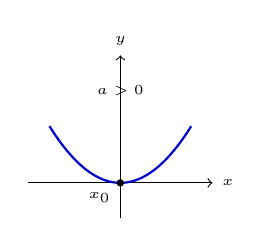
\begin{tikzpicture}[scale=0.9]
    \draw[->] (-1.3,0) -- (1.3,0) node[right] {\tiny $x$};
    \draw[->] (0,-0.5) -- (0,1.8) node[above] {\tiny $y$};
    \draw[domain=-1:1,smooth,variable=\x,blue!80!black,thick] plot ({\x},{0.8*\x*\x});
    \fill (0,0) circle (1.5pt) node[below left] {\tiny $x_0$};
    \node at (0,1.3) {\tiny $a>0$};
\end{tikzpicture}%
\hspace{2mm}%
% Hình 2: a < 0
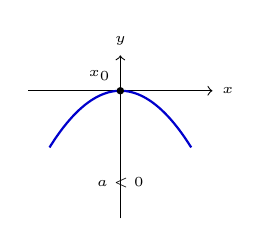
\begin{tikzpicture}[scale=0.9]
    \draw[->] (-1.3,0) -- (1.3,0) node[right] {\tiny $x$};
    \draw[->] (0,-1.8) -- (0,0.5) node[above] {\tiny $y$};
    \draw[domain=-1:1,smooth,variable=\x,blue!80!black,thick] plot ({\x},{-0.8*\x*\x});
    \fill (0,0) circle (1.5pt) node[above left] {\tiny $x_0$};
    \node at (0,-1.3) {\tiny $a<0$};
\end{tikzpicture}
\end{minipage}
\end{tcolorbox}

% Trường hợp 3
\begin{tcolorbox}[colback=blue!3!white,colframe=blue!60!black,title=\textbf{Trường hợp 3: Biệt thức $\Delta > 0$},arc=2mm,boxrule=0.5mm]
Phương trình $f(x) = 0$ có hai nghiệm phân biệt $x_1, x_2$ ($x_1 < x_2$). Quy tắc xét dấu \textbf{"trong trái, ngoài cùng"}:
\begin{itemize}[leftmargin=*]
    \item \textbf{Bên trong khoảng hai nghiệm} ($x_1 < x < x_2$): $f(x)$ mang dấu \textbf{trái} dấu hệ số $a$.
    \item \textbf{Bên ngoài khoảng hai nghiệm} ($x < x_1$ hoặc $x > x_2$): $f(x)$ mang dấu \textbf{cùng} dấu hệ số $a$.
\end{itemize}
\vspace{0.1cm}
\begin{minipage}[c]{0.52\textwidth}
\textbf{Ý nghĩa hình học:} Parabol cắt trục hoành tại hai điểm phân biệt có hoành độ $x_1, x_2$, tạo sự đan xen về dấu.
\end{minipage}%
\begin{minipage}[c]{0.48\textwidth}
\centering
% Hình 1: a > 0
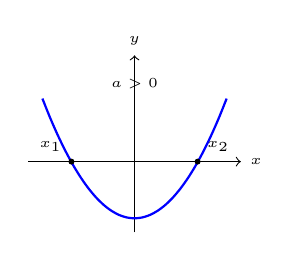
\begin{tikzpicture}[scale=0.9]
    \draw[->] (-1.5,0) -- (1.5,0) node[right] {\tiny $x$};
    \draw[->] (0,-1) -- (0,1.5) node[above] {\tiny $y$};
    \draw[domain=-1.3:1.3,smooth,variable=\x,blue,thick] plot ({\x},{\x*\x - 0.8});
    \fill (-0.89,0) circle (1.2pt) node[above left] {\tiny $x_1$};
    \fill (0.89,0) circle (1.2pt) node[above right] {\tiny $x_2$};
    \node at (0,1.1) {\tiny $a>0$};
\end{tikzpicture}%
\hspace{2mm}%
% Hình 2: a < 0
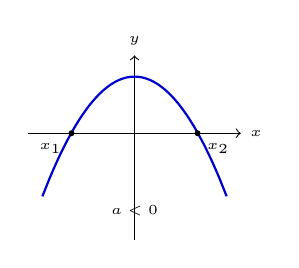
\begin{tikzpicture}[scale=0.9]
    \draw[->] (-1.5,0) -- (1.5,0) node[right] {\tiny $x$};
    \draw[->] (0,-1.5) -- (0,1.1) node[above] {\tiny $y$};
    \draw[domain=-1.3:1.3,smooth,variable=\x,blue!80!black,thick] plot ({\x},{0.8 - \x*\x});
    \fill (-0.89,0) circle (1.2pt) node[below left] {\tiny $x_1$};
    \fill (0.89,0) circle (1.2pt) node[below right] {\tiny $x_2$};
    \node at (0,-1.1) {\tiny $a<0$};
\end{tikzpicture}
\end{minipage}
\end{tcolorbox}

\vspace{0.2cm}
\noindent\textbf{Quy tắc xác định tập nghiệm của bất phương trình:}
Từ định lý cốt lõi nêu trên, quy trình giải một bất đẳng thức bậc hai một ẩn trong thực tế thường trải qua ba bước đơn giản:

\begin{enumerate}[leftmargin=*]
    \item \textbf{Bước 1:} Tính biệt thức $\Delta$ và tìm nghiệm của phương trình $f(x) = 0$ (nếu có).
    \item \textbf{Bước 2:} Dựa vào dấu của $a$ và quy tắc tương ứng với $\Delta$ để lập bảng xét dấu cho $f(x)$ trên toàn bộ trục số.
    \item \textbf{Bước 3:} Đối chiếu với chiều của bất đẳng thức ban đầu để chọn ra các khoảng giá trị của $x$ phù hợp, kết luận tập nghiệm $S$.
\end{enumerate}

Khả năng phân tích và xét dấu nhạy bén này chính là công cụ tư duy định lượng mạnh mẽ, giúp chúng ta tính toán chính xác các khoảng giá trị an toàn trong các bài toán thực tiễn ở những chương tiếp theo.

\newpage

\section*{\centering CHƯƠNG II: ỨNG DỤNG TRONG KINH DOANH NHỎ VÀ QUẢN LÝ TÀI CHÍNH GIA ĐÌNH}

Trong môi trường kinh doanh thực tế, việc đưa ra quyết định về giá bán luôn là một bài toán hóc búa đối với các chủ doanh nghiệp nhỏ. Nếu định giá quá thấp, dù bán được số lượng lớn nhưng biên độ lợi nhuận lại mỏng manh, không đủ bù đắp chi phí vận hành. Ngược lại, nếu định giá quá cao, sản lượng tiêu thụ sẽ sụt giảm mạnh khiến tổng doanh thu lao dốc. Đây chính là lúc bất đẳng thức bậc hai phát huy sức mạnh, giúp người kinh doanh tìm ra một "khoảng giá an toàn" để đảm bảo đạt được mức lợi nhuận kỳ vọng.

\subsection*{2.1. Mô hình định giá bán hàng trà sữa đạt lợi nhuận mục tiêu}

Giả sử một cửa hàng trà sữa nhỏ đang kinh doanh một dòng sản phẩm đồ uống đặc trưng. Qua quá trình hạch toán, chủ quán nhận thấy với mức giá hiện tại, mỗi cốc trà sữa mang lại mức lợi nhuận ròng là $15$ nghìn đồng, và trung bình mỗi ngày cửa hàng bán được $120$ cốc. Như vậy, mức lợi nhuận tổng cộng mỗi ngày đang là $15 \times 120 = 1800$ (nghìn đồng).

Nhằm đối phó với tình hình trượt giá của nguyên vật liệu, chủ quán dự định tăng giá bán. Tuy nhiên, qua khảo sát thị trường, người quản lý ước tính được một quy luật biến động nhu cầu: cứ mỗi lần tăng giá thêm $1$ nghìn đồng, số lượng trà sữa bán ra trong ngày sẽ giảm đi $3$ cốc do khách hàng chuyển sang các quán đối thủ.

\textbf{Thiết lập mô hình toán học:} \\
Gọi $x$ (nghìn đồng) là mức giá tăng thêm trên mỗi cốc trà sữa ($x > 0$). Dựa vào dữ kiện trên, ta có thể biểu diễn các đại lượng kinh doanh theo biến số $x$ như sau:
\begin{itemize}
    \item Lợi nhuận ròng thu được trên mỗi cốc sau khi tăng giá: $15 + x$ (nghìn đồng).
    \item Sản lượng tiêu thụ trung bình mỗi ngày tương ứng: $120 - 3x$ (cốc).
\end{itemize}
Từ đó, tổng lợi nhuận mỗi ngày của cửa hàng, ký hiệu là $L(x)$, được tính bằng tích của lợi nhuận trên mỗi cốc và sản lượng tiêu thụ:
\begin{align*}
    L(x) &= (15 + x)(120 - 3x) \\
    L(x) &= 1800 - 45x + 120x - 3x^2 \\
    L(x) &= -3x^2 + 75x + 1800 \quad \text{(nghìn đồng)}
\end{align*}
Đây chính là một hàm số bậc hai với hệ số $a = -3 < 0$, đồ thị của nó là một parabol có bề lõm hướng xuống dưới.

\textbf{Giải bài toán tối ưu hóa theo mục tiêu:} \\
Sau khi tính toán các chi phí cố định (mặt bằng, điện nước, nhân viên), chủ quán đặt ra mục tiêu lợi nhuận mỗi ngày phải đạt ít nhất $2250$ nghìn đồng mới có thể duy trì hoạt động kinh doanh bền vững và có tích lũy. Bài toán định giá lúc này được chuyển thành việc giải bất đẳng thức:
\[ L(x) \ge 2250 \]
Thay hàm $L(x)$ vào bất đẳng thức, ta có:
\[ -3x^2 + 75x + 1800 \ge 2250 \]
\[ -3x^2 + 75x - 450 \ge 0 \]
Để đơn giản hóa, ta chia cả hai vế cho $-3$ (lưu ý phải đổi chiều bất đẳng thức):
\[ x^2 - 25x + 150 \le 0 \]
Xét tam thức bậc hai $f(x) = x^2 - 25x + 150$. Ta tính được biệt thức $\Delta = (-25)^2 - 4(1)(150) = 625 - 600 = 25 > 0$. Phương trình $f(x) = 0$ có hai nghiệm phân biệt là:
\[ x_1 = \frac{25 - 5}{2} = 10 \quad \text{và} \quad x_2 = \frac{25 + 5}{2} = 15 \]
Vì hệ số $a$ của tam thức $f(x)$ bằng $1 > 0$, áp dụng định lý xét dấu "trong trái, ngoài cùng", tam thức mang dấu âm (nhỏ hơn hoặc bằng $0$) khi biến $x$ nằm trong khoảng giữa hai nghiệm. Do đó, tập nghiệm của bất đẳng thức là:
\[ 10 \le x \le 15 \]
\textbf{Kết luận ý nghĩa thực tiễn:} \\
Kết quả giải bất đẳng thức chỉ ra rằng, để đạt được mức lợi nhuận kỳ vọng là $2250$ nghìn đồng/ngày, chủ quán cần tăng giá bán mỗi cốc trà sữa thêm từ $10$ nghìn đồng đến $15$ nghìn đồng. Đây chính là "miền giá bán an toàn". Nếu tăng giá ít hơn $10$ nghìn, biên lợi nhuận trên mỗi cốc không đủ lớn để đẩy tổng lợi nhuận lên mốc mục tiêu. Ngược lại, nếu tham lam tăng giá vượt quá $15$ nghìn, lượng khách hàng sụt giảm quá mạnh sẽ khiến doanh thu tổng bị kéo xuống dưới mức an toàn.

Đặc biệt, nếu phân tích thêm về đỉnh của parabol, ta có hoành độ đỉnh $h = -\frac{75}{2(-3)} = 12.5$. Nghĩa là, mức lợi nhuận lớn nhất mà cửa hàng có thể đạt được xảy ra khi tăng giá thêm đúng $12.5$ nghìn đồng. Khi đó, lợi nhuận tối đa đạt được là $L(12.5) = 2268.75$ nghìn đồng/ngày.

\subsection*{2.2. Trực quan hóa mô hình kinh doanh bằng mã LaTeX}

Để mang lại cái nhìn trực quan nhất cho người đọc, phần dưới đây sử dụng mã lệnh PGFPlots trong hệ thống LaTeX nhằm phác họa đồ thị của hàm lợi nhuận $L(x)$. Đồ thị thể hiện rõ hình dáng parabol, đường ngưỡng lợi nhuận mục tiêu nằm ngang ở mức $2250$ nghìn đồng, và vùng tô đậm phản ánh miền quyết định giá bán an toàn.

\begin{figure}[htbp]
\centering
\begin{tikzpicture}
\begin{axis}[
    width=13cm, height=8.5cm,
    axis lines=left,
    xmin=0, xmax=25,
    ymin=1500, ymax=2450, % Tăng ymax lên 2450 để đỉnh Parabol có khoảng trống thoáng
    xlabel={Mức giá tăng thêm $x$ (nghìn VNĐ)},
    ylabel={Tổng lợi nhuận $L(x)$ (nghìn VNĐ)},
    grid=both,
    minor tick num=1,
    legend pos=south east,
    legend cell align={left} % Căn trái chữ trong hộp chú thích
]

% Tô màu vùng nghiệm an toàn (dùng forget plot để không làm lệch màu chú thích)
\addplot [fill=green!20, draw=none, domain=10:15, forget plot] {-3*x^2 + 75*x + 1800} \closedcycle;
\addplot [fill=white, draw=none, domain=10:15, forget plot] {2250} \closedcycle;

% 1. Đường cong lợi nhuận (Nét liền màu xanh dương)
\addplot [draw=blue, thick, domain=0:25, samples=100, smooth] {-3*x^2 + 75*x + 1800};
\addlegendentry{Đường cong lợi nhuận $L(x)$}

% 2. Đường mục tiêu lợi nhuận (Nét đứt màu đỏ)
\addplot [draw=red, dashed, line width=1pt, domain=0:25, samples=2] {2250};
\addlegendentry{Mục tiêu lợi nhuận (2250)}

% Đánh dấu hai điểm biên (Dùng forget plot)
\addplot[mark=*, mark options={fill=red, draw=red}, only marks, forget plot] coordinates {(10,2250) (15,2250)};

% Tách tọa độ hai điểm biên sang hai bên (above left và above right) để không bị dính chữ
\node[above left, font=\small] at (axis cs:10, 2250) {$(10; 2250)$};
\node[above right, font=\small] at (axis cs:15, 2250) {$(15; 2250)$};

% Đánh dấu và hiển thị đỉnh Parabol ở chính giữa bên trên
\addplot[mark=*, mark options={fill=blue, draw=blue}, only marks, forget plot] coordinates {(12.5, 2268.75)};
\node[above=0.2cm, font=\small\bfseries] at (axis cs:12.5, 2268.75) {$V(12.5; 2268.75)$};

% Nhãn vùng an toàn
\node[align=center, text=teal, font=\bfseries] at (axis cs:12.5, 2000) {Vùng định giá\\an toàn};

\end{axis}
\end{tikzpicture}
\caption{Đồ thị mô phỏng sự biến thiên của lợi nhuận theo mức tăng giá bán.}
\label{fig:business_model}
\end{figure}

Thông qua sự kết hợp giữa lập luận đại số và biểu đồ hình học trực quan, bài toán quản lý tài chính kinh doanh nhỏ không còn là những phép đoán mò cảm tính, mà đã trở thành một bài toán định lượng có đáp án chính xác và khoa học.

\clearpage

\section*{\centering CHƯƠNG III: ỨNG DỤNG TRONG THỂ THAO DÂN DÃ VÀ AN TOÀN GIAO THÔNG}

Vượt ra khỏi các con số tài chính khô khan, bất đẳng thức bậc hai còn chứng minh được sự hiện diện mạnh mẽ trong việc mô phỏng các quy luật chuyển động của vật lý. Từ đường bay uốn lượn của một quả cầu lông trên sân tập cho đến những phép tính sinh tử về khoảng cách phanh xe trên đường cao tốc, tất cả đều có thể được lượng hóa và kiểm soát thông qua các hàm số và bất đẳng thức bậc hai.

\subsection*{3.1. Bài toán quỹ đạo phát cầu lông qua lưới}

Trong bộ môn cầu lông, quỹ đạo bay của quả cầu sau khi rời mặt vợt luôn tạo thành một đường cong parabol do chịu tác dụng của trọng lực. Một cú phát cầu được xem là hợp lệ nếu quả cầu phải bay vượt qua được mép trên của tấm lưới chắn ở giữa sân và rơi đúng vào phạm vi ranh giới của phần sân đối phương.

\textbf{Thiết lập mô hình quỹ đạo:} \\
Giả sử một vận động viên thực hiện cú đánh cầu. Chọn hệ trục tọa độ $Oxy$ với gốc tọa độ nằm trên mặt đất ngay dưới chân vận động viên. Gọi $x$ (mét) là khoảng cách bay theo phương ngang và $h(x)$ (mét) là chiều cao của quả cầu so với mặt đất. Dựa trên các thông số về lực đánh và góc phát, phương trình quỹ đạo bay của quả cầu được các chuyên gia thể thao mô phỏng bằng hàm số bậc hai:
\[ h(x) = -0.1x^2 + 0.8x + 1.2 \quad (x \ge 0) \]

\textbf{Điều kiện vượt qua lưới:} \\
Theo tiêu chuẩn thi đấu, tấm lưới được đặt cách vị trí người phát một khoảng là $4\text{m}$ (tức $x = 4$), và chiều cao của mép trên tấm lưới là $1.524\text{m}$. Để quả cầu không bị vướng lưới, chiều cao quỹ đạo tại vị trí $x = 4$ phải lớn hơn chiều cao lưới, tương đương với việc thỏa mãn bất đẳng thức:
\[ h(4) > 1.524 \]
Thay giá trị $x = 4$ vào phương trình quỹ đạo, ta có:
\[ h(4) = -0.1(4)^2 + 0.8(4) + 1.2 = -1.6 + 3.2 + 1.2 = 2.8\text{m} \]
Vì $2.8\text{m} > 1.524\text{m}$, quả cầu hoàn toàn vượt qua lưới một cách an toàn với khoảng cách rất thoáng.

\textbf{Xác định điểm rơi của quả cầu:} \\
Bài toán tiếp theo là xác định xem quả cầu sẽ rơi chạm mặt đất ở khoảng cách bao xa. Quả cầu chạm đất khi chiều cao $h(x) = 0$. Vùng không gian quả cầu bay trên không tương ứng với bất đẳng thức $h(x) \ge 0$. Ta xét phương trình giao điểm với mặt đất:
\[ -0.1x^2 + 0.8x + 1.2 = 0 \]
Tính biệt thức thu gọn $\Delta' = 0.4^2 - (-0.1)(1.2) = 0.16 + 0.12 = 0.28 > 0$. Phương trình có hai nghiệm:
\[ x_1 = \frac{-0.4 - \sqrt{0.28}}{-0.1} = 4 + \sqrt{28} \approx 9.29\text{m} \]
\[ x_2 = \frac{-0.4 + \sqrt{0.28}}{-0.1} = 4 - \sqrt{28} \approx -1.29\text{m} \text{ (loại vì } x \ge 0) \]
Như vậy, quả cầu sẽ bay trên không trong khoảng $0 \le x < 9.29$ và chạm đất ở khoảng cách xấp xỉ $9.29\text{m}$ tính từ vị trí phát. Nếu đường biên ngang của sân đối phương nằm ở mốc $10\text{m}$, điểm rơi $9.29\text{m}$ chứng tỏ đây là một pha phát cầu hợp lệ và ghi điểm.

\subsection*{3.2. Tính toán khoảng cách phanh xe an toàn trong giao thông}

Chuyển sang một vấn đề mang tính sống còn hơn: an toàn giao thông đô thị. Khi một tài xế phát hiện chướng ngại vật và quyết định đạp phanh, chiếc xe không dừng lại ngay lập tức. Tổng quãng đường dừng xe là tổng hợp của hai yếu tố: quãng đường xe đi được trong thời gian tài xế phản xạ và quãng đường trượt vật lý của bánh xe khi hệ thống phanh hoạt động. Cả hai yếu tố này đều phụ thuộc vào vận tốc di chuyển ban đầu của xe.

\textbf{Thiết lập mô hình dừng xe:} \\
Các kỹ sư giao thông đã xây dựng một hàm số thực nghiệm để tính toán tổng quãng đường dừng xe an toàn $S(v)$ (tính bằng mét) dựa trên vận tốc $v$ (tính bằng km/h) như sau:
\[ S(v) = 0.005v^2 + 0.2v \quad (v > 0) \]
Trong đó, thành phần bậc nhất $0.2v$ đại diện cho quãng đường phản xạ, còn thành phần bậc hai $0.005v^2$ đại diện cho lực phanh cơ học và quán tính.

\textbf{Lập và giải bất đẳng thức an toàn:} \\
Giả sử vào một ngày sương mù, tầm nhìn của tài xế bị hạn chế ở mức tối đa là $40\text{m}$. Nếu phát hiện một khúc cây đổ ngang đường ở khoảng cách này, tài xế phải phanh gấp. Để xe dừng lại kịp thời trước khi tông vào chướng ngại vật, tổng quãng đường dừng xe phải thỏa mãn bất đẳng thức:
\[ S(v) \le 40 \]
\[ \iff 0.005v^2 + 0.2v - 40 \le 0 \]
Xét tam thức $f(v) = 0.005v^2 + 0.2v - 40$. Tính biệt thức thu gọn $\Delta' = (0.1)^2 - 0.005(-40) = 0.01 + 0.2 = 0.21 > 0$. Phương trình $f(v) = 0$ có nghiệm dương là:
\[ v = \frac{-0.1 + \sqrt{0.21}}{0.005} \approx \frac{-0.1 + 0.4582}{0.005} \approx 71.65\text{km/h} \]
Theo định lý xét dấu, để bất đẳng thức $\le 0$ (với hệ số $a = 0.005 > 0$), biến $v$ phải nằm trong khoảng giữa hai nghiệm. Phối hợp với điều kiện thực tế $v > 0$, ta có tập nghiệm:
\[ 0 < v \le 71.65\text{km/h} \]
Kết quả này mang đến một chỉ dẫn an toàn vô giá: Trong điều kiện tầm nhìn $40\text{m}$, tài xế tuyệt đối không được phép điều khiển xe vượt quá giới hạn $71.65\text{km/h}$. Nếu đi nhanh hơn mốc này, quán tính bậc hai sẽ khiến chiếc xe trượt dài vượt quá $40\text{m}$, dẫn đến tai nạn không thể tránh khỏi.

\subsection*{3.3. Trực quan hóa bằng mã LaTeX}

Dưới đây là phần mô phỏng đồ họa cho cả hai bài toán trên bằng gói lệnh PGFPlots, giúp hình dung rõ nét đường cong vật lý cũng như ranh giới an toàn.

\begin{figure}[htbp]
\centering
\begin{tikzpicture}
\begin{axis}[
    width=14cm, height=6.5cm,
    axis lines=left,
    xmin=0, xmax=11,
    ymin=0, ymax=3.5,
    xlabel={Khoảng cách ngang $x$ (m)},
    ylabel={Chiều cao quả cầu $h(x)$ (m)},
    grid=both,
    minor tick num=1,
    legend pos=north east
]
% Quỹ đạo quả cầu
\addplot [draw=blue, thick, domain=0:9.29, samples=100, smooth] {-0.1*x^2 + 0.8*x + 1.2};
\addlegendentry{Quỹ đạo cầu}

% Lưới chắn
\draw[draw=red, line width=2pt] (axis cs:4,0) -- (axis cs:4,1.524);
\node[right, font=\small, text=red] at (axis cs:4.1, 0.7) {Lưới ($1.52\text{m}$)};

% Điểm rơi
\addplot[mark=*, mark options={fill=red}, only marks] coordinates {(9.29,0)};
\node[above left, font=\small] at (axis cs:9.29, 0) {Điểm chạm đất ($9.29\text{m}$)};
\end{axis}
\end{tikzpicture}
\caption{Mô phỏng quỹ đạo bay của quả cầu lông qua lưới chắn.}
\end{figure}

\vspace{0.5cm}

\begin{figure}[htbp]
\centering
\begin{tikzpicture}
\begin{axis}[
    width=14cm, height=6.5cm,
    axis lines=left,
    xmin=0, xmax=100,
    ymin=0, ymax=70,
    xlabel={Vận tốc xe $v$ (km/h)},
    ylabel={Quãng đường phanh $S(v)$ (m)},
    grid=both,
    minor tick num=1,
    legend pos=north west,
    legend cell align={left}
]
% Đường cong dừng xe
\addplot [draw=orange, thick, domain=0:100, samples=100, smooth] {0.005*x^2 + 0.2*x};
\addlegendentry{Quãng đường phanh}

% Vùng giới hạn an toàn (tô màu)
\addplot [fill=green!20, draw=none, domain=0:71.65, forget plot] {40} \closedcycle;
\addplot [fill=white, draw=none, domain=0:71.65, forget plot] {0.005*x^2 + 0.2*x} \closedcycle;

% Ngưỡng tầm nhìn
\addplot [draw=red, dashed, thick, domain=0:100, samples=2] {40};
\addlegendentry{Tầm nhìn tối đa ($40\text{m}$)}

% Điểm giao cắt (vận tốc giới hạn)
\addplot[mark=*, mark options={fill=red}, only marks, forget plot] coordinates {(71.65,40)};
\draw[dashed, thick] (axis cs:71.65,40) -- (axis cs:71.65,0);
\node[below, font=\bfseries] at (axis cs:71.65, 0) {$71.65$};
\node[above left, font=\small] at (axis cs:71.65, 40) {Giới hạn an toàn};
\end{axis}
\end{tikzpicture}
\caption{Đồ thị liên hệ giữa vận tốc và quãng đường phanh an toàn.}
\end{figure}

\clearpage

\section*{\centering CHƯƠNG IV: ỨNG DỤNG TRONG THIẾT KẾ CẢNH QUAN VÀ KIẾN TRÚC DÂN DỤNG}

Kiến trúc và thiết kế cảnh quan không chỉ đòi hỏi con mắt thẩm mỹ mà còn cần sự chính xác tuyệt đối của hình học và đại số. Khi quy hoạch không gian, các kiến trúc sư thường xuyên phải đối mặt với bài toán cân bằng: làm sao để bố trí lối đi, kết cấu chịu lực hay mái che mà không xâm phạm vào không gian sinh hoạt cốt lõi. Bất đẳng thức bậc hai cung cấp một phương pháp luận sắc bén để thiết lập các giới hạn không gian này.

\subsection*{4.1. Quy hoạch lối đi sân vườn}

Một gia đình có mảnh đất trống hình chữ nhật phía trước nhà với kích thước chiều dài là $10\text{m}$ và chiều rộng là $8\text{m}$. Chủ nhà muốn thiết kế một lối đi lát gạch xung quanh mép trong của mảnh đất, phần diện tích còn lại ở chính giữa sẽ được trồng cỏ và hoa. Để đảm bảo tính thẩm mỹ đồng bộ, lối đi này phải có bề rộng bằng nhau ở tất cả các cạnh.

\textbf{Thiết lập mô hình toán học:} \\
Gọi $x$ (mét) là bề rộng của lối đi ($x > 0$). Vì lối đi chạy dọc theo cả hai bên chiều dài và hai bên chiều rộng, nên kích thước của phần sân cỏ hình chữ nhật bên trong sẽ bị thu hẹp lại. Cụ thể:
\begin{itemize}
    \item Chiều dài phần sân cỏ: $10 - 2x$ (m).
    \item Chiều rộng phần sân cỏ: $8 - 2x$ (m).
\end{itemize}
Để phần sân cỏ tồn tại trên thực tế, kích thước phải là số dương, tức là $10 - 2x > 0$ và $8 - 2x > 0$. Từ đó ta có điều kiện vật lý của biến: $0 < x < 4$.

Diện tích phần trồng cỏ, ký hiệu là $S(x)$, được tính bằng:
\[ S(x) = (10 - 2x)(8 - 2x) = 80 - 20x - 16x + 4x^2 = 4x^2 - 36x + 80 \quad (\text{m}^2) \]

\textbf{Bài toán giới hạn diện tích:} \\
Chủ nhà yêu cầu diện tích phần trồng cỏ và hoa không được nhỏ hơn $48\text{m}^2$ để có đủ không gian tổ chức tiệc trà ngoài trời. Yêu cầu này dẫn đến bất đẳng thức:
\[ S(x) \ge 48 \]
\[ 4x^2 - 36x + 80 \ge 48 \]
\[ 4x^2 - 36x + 32 \ge 0 \]
Chia cả hai vế cho $4$, ta được bất đẳng thức thu gọn:
\[ x^2 - 9x + 8 \ge 0 \]
Xét tam thức $f(x) = x^2 - 9x + 8$. Phương trình $f(x) = 0$ có tổng các hệ số $1 - 9 + 8 = 0$ nên dễ dàng nhẩm được hai nghiệm là $x_1 = 1$ và $x_2 = 8$. Vì hệ số $a = 1 > 0$, áp dụng quy tắc "trong trái, ngoài cùng", tập nghiệm của bất đẳng thức là:
\[ x \le 1 \quad \text{hoặc} \quad x \ge 8 \]
Kết hợp với điều kiện thực tế của mảnh đất là $0 < x < 4$, ta loại bỏ trường hợp $x \ge 8$. 
Kết luận: $0 < x \le 1$. 

Như vậy, để giữ lại ít nhất $48\text{m}^2$ cho thảm cỏ, bề rộng của lối đi sân vườn tối đa chỉ được phép là $1\text{m}$. Nếu lát lối đi rộng hơn, diện tích mảng xanh sẽ bị bóp nghẹt dưới mức yêu cầu.

\subsection*{4.2. Tính toán không gian lọt lòng của mái che vòm parabol}

Tại một bãi đậu xe, người ta xây dựng một mái che có mặt cắt hình parabol. Mái che này có chiều cao tại đỉnh (điểm cao nhất so với mặt đất) là $4.5\text{m}$ và bề rộng của phần chân đế trên mặt đất là $6\text{m}$. 

\textbf{Thiết lập phương trình mặt cắt:} \\
Gắn hệ trục tọa độ $Oxy$ sao cho gốc $O$ nằm trên mặt đất ngay chính giữa mái che. Khi đó, mặt đất tương ứng với trục hoành ($y = 0$), trục tung đi qua đỉnh mái che. Đỉnh của parabol sẽ có tọa độ là $V(0; 4.5)$. Phương trình mái che có dạng $y = ax^2 + 4.5$.
Vì chân mái che rộng $6\text{m}$, nên nó cắt trục hoành tại hai điểm có hoành độ là $x = -3$ và $x = 3$. Thay tọa độ $(3; 0)$ vào phương trình, ta có:
\[ 0 = a(3)^2 + 4.5 \implies 9a = -4.5 \implies a = -0.5 \]
Vậy phương trình của vòm mái che là: $y = -0.5x^2 + 4.5$ (với $-3 \le x \le 3$).

\textbf{Kiểm tra giới hạn an toàn cho phương tiện:} \\
Một chiếc xe tải giao hàng có chiều cao tổng thể là $2.5\text{m}$ muốn lùi vào vị trí dưới mái che này. Câu hỏi đặt ra là: Chiều rộng tối đa của chiếc xe tải có thể là bao nhiêu để khi đậu ở vị trí chính giữa, các góc phía trên của thùng xe không bị va quẹt vào trần mái che?

Gọi $2x$ (mét) là chiều rộng của chiếc xe (với $x > 0$ là nửa chiều rộng tính từ tâm bãi đậu). Để xe không chạm mái, chiều cao của mái che tại ranh giới hai bên thùng xe (tức tại hoành độ $x$ và $-x$) phải lớn hơn hoặc bằng chiều cao của xe tải. Ta có bất đẳng thức:
\[ -0.5x^2 + 4.5 \ge 2.5 \]
\[ -0.5x^2 + 2 \ge 0 \]
Nhân cả hai vế cho $-2$ (đổi chiều bất đẳng thức):
\[ x^2 - 4 \le 0 \]
Tam thức $x^2 - 4$ có hai nghiệm là $-2$ và $2$. Để biểu thức nhỏ hơn hoặc bằng $0$, $x$ phải nằm trong khoảng:
\[ -2 \le x \le 2 \]
Do $x$ là khoảng cách nửa chiều rộng bề ngang, bề rộng tối đa của xe tải là $2x = 2 \times 2 = 4\text{m}$.
Kết luận: Bất kỳ chiếc xe tải nào cao $2.5\text{m}$ nhưng có bề ngang hẹp hơn hoặc bằng $4\text{m}$ đều có thể đậu an toàn dưới vòm mái che này. 

\subsection*{4.3. Biểu diễn hình học các mô hình thiết kế}

Dưới đây là sơ đồ mặt bằng sân vườn và mặt cắt đứng của mái che vòm, được mô phỏng trực tiếp bằng mã lệnh đồ họa để mang lại góc nhìn trực quan cho các bài toán kiến trúc trên.

\begin{figure}[htbp]
\centering
\begin{tikzpicture}
% Vẽ ranh giới ngoài của mảnh đất (10x8)
\draw[thick, fill=gray!20] (0,0) rectangle (10,8);

% Vẽ ranh giới trong của bãi cỏ (bề rộng lối đi x = 1, nên kích thước trong là 8x6)
\draw[thick, fill=green!30, dashed] (1,1) rectangle (9,7);

% Ghi chú kích thước ngoài
\draw[<->] (0,-0.5) -- (10,-0.5) node[midway, fill=white] {Chiều dài đất $10\text{m}$};
\draw[<->] (-0.5,0) -- (-0.5,8) node[midway, fill=white, rotate=90] {Chiều rộng đất $8\text{m}$};

% Ghi chú kích thước sân cỏ
\node[align=center, font=\large\bfseries, text=teal] at (5,4) {Sân cỏ \& Hoa \\ $S \ge 48\text{m}^2$};

% Ghi chú lối đi x
\draw[<->, thick, red] (0, 4) -- (1, 4) node[midway, above, font=\small] {$x$};
\draw[<->, thick, red] (5, 8) -- (5, 7) node[midway, right, font=\small] {$x$};

\node[below, font=\itshape] at (5,-1.2) {(a) Sơ đồ quy hoạch sân vườn (mặt bằng)};
\end{tikzpicture}
\end{figure}

\vspace{0.5cm}

\begin{figure}[htbp]
\centering
\begin{tikzpicture}
\begin{axis}[
    width=14cm, height=7cm,
    axis lines=center,
    xmin=-4, xmax=4,
    ymin=-0.5, ymax=5.5,
    xlabel={$x$ (m)},
    ylabel={$y$ (m)},
    grid=both,
    minor tick num=1
]
% Vẽ vòm mái che
\addplot [draw=blue, ultra thick, domain=-3:3, samples=100, smooth] {-0.5*x^2 + 4.5};
\addlegendentry{Mái che vòm}

% Vẽ chiếc xe tải (hình chữ nhật cao 2.5m, rộng 4m tức từ -2 đến 2)
\addplot [fill=red!20, draw=red, thick, forget plot] coordinates {(-2,0) (2,0) (2,2.5) (-2,2.5) (-2,0)};

% Điểm nguy hiểm (Góc xe tải chạm mái che)
\addplot[mark=*, mark options={fill=red}, only marks] coordinates {(-2,2.5) (2,2.5)};
\node[above left, font=\small, text=red] at (axis cs:-2, 2.5) {Góc chạm $(-2; 2.5)$};
\node[above right, font=\small, text=red] at (axis cs:2, 2.5) {Góc chạm $(2; 2.5)$};

% Ghi chú kích thước xe
\node[align=center, font=\bfseries] at (axis cs:0, 1.25) {Thùng xe tải\\(Rộng $4\text{m}$, Cao $2.5\text{m}$)};
\end{axis}
\end{tikzpicture}
\caption{Mô phỏng mặt cắt kiến trúc và giới hạn an toàn.}
\end{figure}

\clearpage

\section*{\centering KẾT LUẬN}

Nghiên cứu đã khẳng định bất đẳng thức bậc hai không phải là những dòng công thức khô khan hay đáp số trừu tượng trên trang sách. Ngược lại, đây là công cụ tư duy định lượng sắc bén, giúp chuyển hóa các vấn đề thực tế phức tạp—từ tính toán biên độ lợi nhuận kinh doanh, ranh giới phanh xe an toàn, đến phân bổ không gian kiến trúc—thành các bài toán tối ưu hóa rõ ràng.   


Trong thực tế, chúng ta hiếm khi tìm kiếm một giá trị tuyệt đối duy nhất. Điều cần thiết cho các quyết định đời sống là một "khoảng an toàn" hay ranh giới linh hoạt để kiểm soát rủi ro. Bất đẳng thức bậc hai đã thực hiện xuất sắc vai trò này khi chuyển đổi những phỏng đoán cảm tính thành các tập nghiệm số học minh bạch, khoa học và đáng tin cậy.   


Việc ứng dụng mã nguồn mở LaTeX cùng gói lệnh PGFPlots đã trực quan hóa các đường cong parabol và miền nghiệm một cách sinh động. Cách tiếp cận này giúp xóa bỏ sự cứng nhắc của đại số thuần túy, mang lại góc nhìn hình học trực diện, hỗ trợ người đọc dễ dàng cảm nhận bản chất và vẻ đẹp ứng dụng của toán học.   


Đề tài góp phần thu hẹp khoảng cách giữa lý thuyết toán học và đời sống thực tế. Đây sẽ là động lực để người học thay đổi lăng kính tiếp cận môn Toán: bớt đi sự trừu tượng, tăng tính ứng dụng và biến kiến thức thành một công cụ hữu ích trong hành trang bước vào đời

\end{document}
